% thesis.tex
% This is the main file, which calls up preamble.tex, frontmatter.tex, and thesis.bib as needed.

% Frontmatter shortcuts; note the extra space at the end, which is unfortunately necessary:
\newcommand\myname{Tsz Leong Chan }
\newcommand\mytitle{COMPUTATIONAL~VERIFICATION OF THE CONE~CONJECTURE } % The graduate division requires this to be in caps.
\newcommand\mydegree{Master of Arts } % change to  Master of Science if applicable
\newcommand\myfield{Mathematics } % e.g., Mathematics
\newcommand\thismonth{December } % graduation month: May / August / December
\newcommand\thisyear{2018 } % e.g., 2014


\documentclass[12pt,oneside]{sfsuthesis}  
%WHEN THESIS IS COMPLETED, CHANGE THE NEXT LINE FROM draft TO final, then the paper will be formatted according to the Graduate Division's guidelines
\usepackage[final]{MAThesisOutputFormat}
\RequirePackage{standalone}


%==========%
% biblatex %
%==========%

\usepackage[backend=biber,style=numeric]{biblatex}
\addbibresource{references.bib}



%=========================%
% CUSTOM PACKAGES GO HERE %
%=========================%


\usepackage{TCbasic}
\usepackage{multicol}
\usepackage{wrapfig}
\usepackage[toc,page]{appendix}
\usepackage{hyperref}


\RequirePackage{listings}



\lstnewenvironment{SAGE}
  {
    \lstset{
        language=Python,
        basicstyle=\ttfamily \small,
        breaklines=true,
        columns=fullflexible,
        showstringspaces=false}
  }
  {
  }




\begin{document}
\thesistitle
% Main body of work:

%--------------------------------------------%
% Packages arranged by : Tsz Timmy Chan	     %
%                 Date : November 26th, 2016%
%--------------------------------------------%

\documentclass{TC}
\usepackage{TCcommon}

\title{TITLE HERE}	% Work Title Here.
\author{Tsz Timmy Chan}	% YOUR NAME HERE 

\usepackage[notes]{TCheader}
\usepackage{TCexamtitle}
%\renewcommand{\benediction}{" " - }
%\renewcommand{\quoteoftheday}{" " \\ - }
\usepackage[style=numeric]{biblatex}
\addbibresource{references.bib}

\title{Computational Verification of the Cone Conjecture}	% Work Title Here.
\author{Tsz Timmy Chan}	% YOUR NAME HERE 

\begin{document}
\chapter{Introduction}

%--------------------------------------------%
% Packages arranged by : Tsz Timmy Chan	     %
%                 Date : November 26th, 2016%
%--------------------------------------------%

\documentclass{TC}
\usepackage{TCcommon}

\title{TITLE HERE}	% Work Title Here.
\author{Tsz Timmy Chan}	% YOUR NAME HERE 

\usepackage[notes]{TCheader}
\usepackage{TCexamtitle}
%\renewcommand{\benediction}{" " - }
%\renewcommand{\quoteoftheday}{" " \\ - }
\begin{document}
%\researchnote{Make citations}

Normal polytopes and rational cones are important objects in integer programming, optimization, combinatorics, and algebraic geometry \cite{GubeladzePolytopesRingsKtheory}. Recently, Bruns, Gubeladze, and Micha\l{}ek \cite{BrunsGubeladzeNormalPolytopes} initiated a novel approach to these discrete-convex objects by introducing partial orders on them. The resulting poset of normal polytopes is a discrete model of the continuum of convex compacta in Euclidean spaces. Understanding properties of this poset is a challenge and only partial results in this direction are known to date. Later, Gubeladze and Micha\l{}ek \cite{GubeladzePosetCones} defined a partial order on the set rational cones. The latter poset seems more amenable to analysis than the poset of normal polytopes. What is important, if the partial order on cones is trivial, i.e., coincides with the inclusion order (the Cone Conjecture), then the cones provide a handle on the poset of normal polytopes via the homogenization map. Gubeladze and Micha\l{}ek were able to prove the Cone Conjecture in dimension 3 and Paffenholz provided some computational evidence in dimension 4.

In this thesis we develop computational methods to analyze the Cone Conjecture in higher dimensions and provide big data in dimensions 4 and 5, far exceeding the computational results by Paffenholz. Namely, we use two specific types of moves inside the poset of cones (the so-called "Bottom Up" and "Top Down" moves) to link two randomly generated cones, one containing the other. The Cone Conjecture states that any such a pair of cones is linked by a chain. The mentioned specific moves often produce such chains. But there are non-terminating examples as well. In order to get a deeper insight into the complexity of the poset of cones, we keep track of the size of Hilbert bases of the intermediate cones and the lengths of pivotal vectors for the bottom-up and top-down moves. The conclusion is that the method used by Gubeladze and Micha\l{}ek to prove the conjecture in dimension 3 is not appropriate in higher dimensions. New ideas, needed to tackle the conjecture in general, may come from the observed strange monotonicity trends in the Hilbert basis size along the chains of bottom-up and top-down moves. 

In Sections 2 and 3, we give a brief introductory exposition on polytopes, cones, normal polytopes and rational cones. Then, in Sections 4 and 5, we give an exposition on the detailed techniques and implemented algorithms, along with many computational results.

%Normal polytopes and rational cones are important objects in integer programming, optimization, combinatorics and algebraic geometry. The study of these sets, along with the natural partial orders on these objects is at the current forefront of research. 


%This thesis attempts to answer a question posed in a recent paper \emph{the Poset of Rational Cones} \cite{GubeladzePosetCones}. Current research on the partially ordered set of rational cones have given results in dimensions two and three, and further explorations by theoretical means is challenging. Thus, we give computational data to give insight into this nortoriously complicated partially ordered set. This partially ordered set is intricately connected with the partially ordered set of normal polytopes, by the way of a homogenization map. 

%In the following sections, we will give a brief introductory exposition on polytopes, cones, normal polytopes and rational cones. Then after, we give an exposition on the detailed techniques used to implement the algorithms described in \cite{GubeladzePosetCones}.


\end{document}
\chapter{Background}

%--------------------------------------------%
% Packages arranged by : Tsz Timmy Chan	     %
%                 Date : November 26th, 2016%
%--------------------------------------------%

\documentclass{TC}
\usepackage{TCcommon}

\title{TITLE HERE}	% Work Title Here.
\author{Tsz Timmy Chan}	% YOUR NAME HERE 

\usepackage[notes]{TCheader}
\usepackage{TCexamtitle}
%\renewcommand{\benediction}{" " - }
%\renewcommand{\quoteoftheday}{" " \\ - }
\begin{document}
In this project, we are interested in pointed, polyhedral rational cones, which are a special case of polyhedra. Here, we will give rigorous definitions, which are the foundations necessary to discuss the computational experimentation. While the following definitions are general and can be applied to any vector space with an inner product, we are in particular interested in $\R^d$.

\section{Polyhedra}

%--------------------------------------------%
% Packages arranged by : Tsz Timmy Chan	     %
%                 Date : November 26th, 2016%
%--------------------------------------------%

\documentclass{TC}
\usepackage{TCcommon}

\title{TITLE HERE}	% Work Title Here.
\author{Tsz Timmy Chan}	% YOUR NAME HERE 

\usepackage[notes]{TCheader}
\usepackage{TCexamtitle}
%\renewcommand{\benediction}{" " - }
%\renewcommand{\quoteoftheday}{" " \\ - }
\begin{document}
First, we begin with the idea of linear subspaces of a vector space. Linear subspace is the set of vectors that vanishes on a linear form $a_1 x_1 + \cdots + a_nx_n = 0$ for some scalar coefficients. In this paper, we are interested when the vector space is $\R^d$. Consider the linear subspace shifted away from the origin; we will arrive at the first major concept we need to build up to the definitions of polyhedra and polytopes: 

\begin{definition}[Affine subspace]
Affine subspaces are the translates of linear subspaces. The dimension of an affine subspace is the dimension of the associated linear subspace. 
\end{definition}
Affine subspaces of dimension 0, 1 and 2 are called points, lines and planes, respectively.

Let $V$ be a vector space and $\alpha : V \to \R$ be an affine form, which is a function given by $\alpha(x) = \lambda(x) + \alpha_0$, with a unique linear operator $\lambda$ on $V$. We define a hyperplane by the following construction \cite{GubeladzePolytopesRingsKtheory}.

\begin{definition}[Affine Hyperplane]
 $$H_\alpha = \{x \in \R^d: \alpha (x) = 0\}$$ A \emph{hyperplane} is the set of vectors in $\R^d$ that vanish on the affine form $\alpha(x)$. A hyperplane is an affine subspace of dimension $d-1$.
 \end{definition}
 
 Thus, when evaluating any point $x \in \R^d$ that is not on the hyperplane, $\alpha(x) > 0$ or $\alpha(x) < 0$. This gives us a sense of partitioning, as the hyperplane will partition the space into two halves.
  Imagine cutting $\R^d$ into two parts using a $(d-1)$-dimensional plane; each of the two parts is an affine halfspace. 

  \begin{definition}[Open and Closed Affine Halfspaces] An open affine halfspace is defined as $$H_\alpha^> = \{ x \in V : \alpha (x) >0\}$$ for some affine form $\alpha(x)$. A closed halfspace $H_\alpha^+$ is defined as the union of $H_\alpha$ and $H_\alpha^>$. \end{definition}
 
 Formally, according to standard graduate texts in mathematics on geometry \cite{GubeladzePolytopesRingsKtheory, Ziegler}, we can define a \emph{polyhedron} as the intersection of halfspaces:
 
\begin{definition}[H-Polyhedron]  A subset $P \subset V$ is called an H-polyhedron if it is the intersection of finitely many closed affine halfspaces. The dimension of the polyhedron is determined by the dimension of the smallest affine subspace containing $P$. If $\dim(P)~=~d$, we call $P$ a $d$-polyhedron.

\end{definition}

As one can imagine, since the H-Polyhedron definition depends on an intersection of halfspaces, there exist special hyperplanes for each H-polyhedron where each hyperplane is formed from the associated halfspaces. Furthermore, there are hyperplanes that "touch" the H-polyhedron, and how they "touch" the H-polyhedron is how we define faces of lower dimensions. An example in $\R^3$ is a cube, which will have 6 facets of dimension 2, 12 faces (edges) of dimension 1, and 8 faces (vertices) of dimension 0. This condition is formalized for higher dimensions as follows: 


\begin{definition}[Support Hyperplane, Face]
A hyperplane $H$ is called a support hyperplane of the polyhedron $P$ if $P$ is contained in one of the two closed halfspaces bounded by $H$, and $H \cap P \neq \emptyset$. 

In particular, the intersection $F= H \cap P$ is a face of $P$, and $H$ is called a support hyperplane associated with $F$. 
\end{definition}

An H-polyhedron is the intersection of finitely many closed halfspaces, and each halfspace is associated with an affine hyperplane; the intersection of these affine hyperplanes and the polytope form the facets, or faces of dimension $d-1$. Other affine hyperplanes may also satisfy the support hyperplane definition, but the intersection may be lower dimensional.

Visually, in $\R^3$, we can imagine support hyperplanes as hyperplanes (in $\R^3$ hyperplanes are simply 2-dimensional planes) that touch the polyhedron's boundary without cutting through the object, and the part of the polytope that the hyperplane "touches" is a face. A 0,1 and $d-1$ dimensional face of a polytope is called a vertex, an edge and a facet, respectively.


\end{document}

\section{Convex Polytopes}

%--------------------------------------------%
% Packages arranged by : Tsz Timmy Chan	     %
%                 Date : November 26th, 2016%
%--------------------------------------------%

\documentclass{TC}
\usepackage{TCcommon}

\title{TITLE HERE}	% Work Title Here.
\author{Tsz Timmy Chan}	% YOUR NAME HERE 

\usepackage[notes]{TCheader}
\usepackage{TCexamtitle}
%\renewcommand{\benediction}{" " - }
%\renewcommand{\quoteoftheday}{" " \\ - }
\begin{document}
The polytopes in this paper are always convex, so first we define convexity and the convex hull of a set.

A set $X \subset \R^d$ is \emph{convex} when between any two points in $X$, the line segment joining the two points is also contained in $X$. More formally:

\begin{definition}[Convex]
A set $X \subset \R^d$ is convex if for every $x, y \in X$:\\ $\{\lambda x + (1-\lambda)y : 0 \leq \lambda \leq 1\} \subset X$. 
\end{definition}

As a remark, the intersection of any convex set is again convex. More importantly for any arbitrary set $K \subset \R^d$, there exists a smallest convex set containing $K$ constructed as the intersection of all the convex sets that contain $K$. Alternatively, one can say that the convex hull of $K$ contains every line segment joining any two  elements in the set $K$.

\begin{definition}[Convex hull]
Given $K \subset \R^d$, the convex hull of $K$, denoted $\mathrm{conv}(K)$, is the smallest convex set that contains $K$:
\begin{align*}
\mathrm{conv}(K) 	&= \bigcap \{X \subset \R^d: K \subseteq X, X \text{ convex}\} \\
					&= \{\lambda_1 x_1 + \cdots + \lambda_n : \{ x_1,\ldots,x_n\} \subseteq K, \lambda_i \geq 0, \sum_{i=1}^n \lambda_i = 1\}.
\end{align*}

\end{definition}

We will explore two different definitions of the polytope; they are unique representations for each polytope and mathematically equivalent through a nontrivial proof. 

\begin{definition}[V-polytope]
A $V$-polytope is the convex hull of a finite set of points in $\R^d$.
\end{definition}

The other definition that depends on the previous section is the halfspace representation of a polytope:

\begin{definition}[H-polytope] An H-polytope is an H-polyhedron that is bounded. Equivalently, an H-polytope $P$ contains no rays of the form $\{x+ty: t \geq 0\}$ for any $x \in P, y \neq 0$. 
\end{definition}

Finally, a \emph{polytope} is a set $P \subseteq \R^d$ which can be represented as a $V$-polytope or a $H$-polytope. Like the definition for the dimension of a polyhedron, the dimension of a polytope is the dimension of the smallest affine subspace that contains this polytope.


\end{document}

\section{Cones}
%--------------------------------------------%
% Packages arranged by : Tsz Timmy Chan	     %
%                 Date : November 26th, 2016%
%--------------------------------------------%

\documentclass{TC}
\usepackage{TCcommon}

\title{TITLE HERE}	% Work Title Here.
\author{Tsz Timmy Chan}	% YOUR NAME HERE 

\usepackage[notes]{TCheader}
\usepackage{TCexamtitle}
%\renewcommand{\benediction}{" " - }
%\renewcommand{\quoteoftheday}{" " \\ - }
\begin{document}
Cones are intimately related to polytopes and polyhedra. In this narrative to discuss the main theorem of polytope theory, we will show how to embed both H-polyhedra and V-polyhedra of dimension $d$ into $\R^{d+1}$ as cones. This intimate relation between cones and polytopes is also the motivation later for the relationship between normal polytopes and rational cones.

 A cone in a vector space (or $\R^d$) is defined as the following:

\begin{definition}[Cone]
A set $C \subset \R^d$ is a cone if for every $ x \in C , \lambda x \in C \text{ for every } \lambda \geq 0$.
\end{definition}

Clearly, the intersection of cones is again a cone, and some trivial cases are the empty set $\{\emptyset\}$ and the whole space $\R^d$.

Given any set $K \subset \R^d$, we are also interested in the smallest cone that contains this set. Similar to the construction of the convex hull, the \emph{conical hull} can be characterized as the intersection of all the cones that contain $K$ or as non-negative linear combinations of all the elements of $K$:

\begin{definition}[Conical hull] Given a set $K \subseteq \R^d$, the conical hull of $K$, denoted $\mathrm{cone}(K)$, is the smallest cone that contains $K$, and 

\begin{align*}
\mathrm(K) &= \bigcap\{C \subseteq \R^d: K \subseteq C, C \text{ is a cone}\}, \\
			&= \{\lambda_1 x_1 + \cdots + \lambda_n x_n : \{ x_1,\ldots,x_k\} \subseteq K, \lambda_i \geq 0\}.
\end{align*}
In particular, we'll be interested in the case when $K$ is a finite set.
\end{definition}

\begin{figure}[h]
\centering
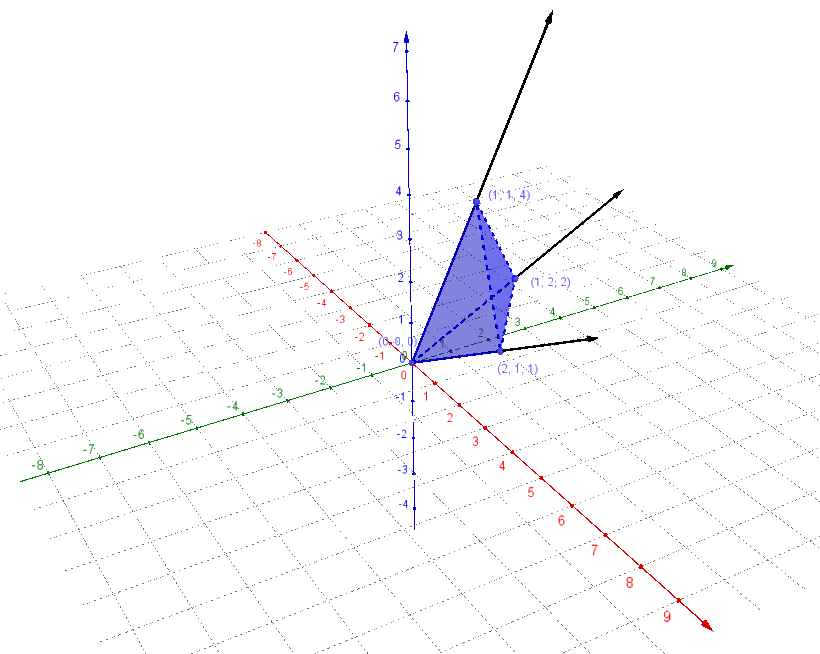
\includegraphics[width=.7\textwidth]{ExampleCone.png}
\caption{Example of $\mathrm{cone}(K)$ for some finite $K \subset \R^3$.}
\end{figure}

The \emph{Minkowski sum} of two sets $P, Q \subseteq \R^d$ is $P+Q = \{ p+q: p \in P, q\in Q\}$. With this operation, we can define a V-polyhedron as the Minkowski sum of the conical hull of a finite set of vectors and the convex hull of another finite set of vectors:

\begin{definition}[V-polyhedron] A \emph{V-polyhedron} denotes any finitely generated convex-conical combination, in other words, a set $P \subset \R^d$ of the form
$$P = \mathrm{conv}(V) + \mathrm{cone}(Y) $$
for some finite sets $V, Y \subset \R^d$.
\end{definition}

From this definition, a \emph{V-polytope} is a bounded \emph{V-polyhedron}. 

To draw the definitive relationship between the unique characterization of the V-polytope as the convex hull of finitely many points and H-polytope as the intersection of finite halfspaces, one strategy is to show that there exists a unique homogenous cone in dimension $d+1$, according to \cite{Ziegler}.

\subsection{Homogenization of Polyhedron} \label{homogenization_map}
The narrative in \cite{Ziegler} introduced the homogenization map, by simply adjoining an extra coordinate to the vectors with the intention to reduce the narrative to show that a V-polyhedra in $\R^d$ is also an H-polyhedra in $\R^d$ by associating a well-defined cone with each type in $\R^{d+1}$ in the following ways, with the goal of embedding the polyhedra in the plane $x_0 = 1$ and forming a cone to represent such a polyhedra without loss of information.

If $P_H$ is some $H$-polyhedron, i.e., $P_H = \{ x \in \R^d : Ax \leq z, A \in \R^{m\times d}, z \in \R^m\}$, we can create a cone in $\R^{d+1}$ by encoding the inequalities $a_i \mathbf x \leq z_i$ into $a_i\mathbf x \leq z_i x_0$ with $x_0 \geq 0$. More specifically, let  

\begin{equation} \label{H-homogenization_map}
C(P_H) =  \begin{bmatrix}
-1 & 0 & \cdots & 0 \\
-z_0 & a_{11} & \cdots & a_{1d} \\
\vdots & \vdots & \ddots & \vdots \\
-z_m & a_{m1} & \cdots & a_{md}
\end{bmatrix} \begin{bmatrix}
x_0 \\ x_1 \\ \vdots \\ x_d
\end{bmatrix} \leq \begin{bmatrix}
0 \\ 0 \\ \vdots \\0
\end{bmatrix}.
\end{equation}
Note that when $x_0 = 1$, we have the polytope $P$ in the plane intersecting $C(P)$, and that $C(P)$ and $P$ are both H-polyhedra.

Similarly, if $P_V$ is some V-polyhedra where $P_V = \mathrm{conv}(U) + \mathrm{cone}(W)$ for some finite sets $U,W \subset \R^d$, we can form a $C(P_V)$ in $\R^{d+1}$ as follows: 

\begin{equation}\label{V-homogenization_map}
C(P_V) = \mathrm{cone}\left(\begin{bmatrix}
1 \\ u_{11} \\ \vdots \\ u_{d1}
\end{bmatrix}, \cdots , 
\begin{bmatrix}
1 \\ u_{1j} \\ \vdots \\ u_{dj}
\end{bmatrix} , \begin{bmatrix}
0 \\ w_{11} \\ \vdots \\ w_{d1}
\end{bmatrix}, \cdots , 
\begin{bmatrix}
0 \\ w_{1k} \\ \vdots \\ w_{dk}
\end{bmatrix}\right),
\end{equation}

The construction creates a cone in $\R^{d+1}$, as the conical hull of these vectors, with the property that $$ P = \left \{ \mathbf x \in \R^d : \begin{bmatrix}
1 \\ \mathbf x
\end{bmatrix} \in C(P)\right \}.$$

And the points at infinity (the part of $P$ that is defined using the conical hull of $Y$) is recorded on the plane $x_0 = 0$.

\begin{theorem}[Main theorem of polytope theory: Cone Version] \label{Cone_Theorem}


A cone $C \subseteq \R^d$ is finitely generated combination of vectors $$ C = \mathrm{cone}(V) \text{ for some finite } V \subset \R^d $$
if and only if it is a finite intersection of closed linear halfspaces
$$ C = \{x \in \R^d : Ax \leq 0\} \text{ for some } A \in \R^{m \times d}\} .$$
\end{theorem}

The proof of this theorem is nontrivial and can be found in Section 1.3 of \cite{Ziegler}. With the information from Theorem \ref{Cone_Theorem}, and the aforementioned construction of cones using V-polyhedra and H-polyhedra, together they imply (through the construction of the homogenization map) the following theorem. 


\begin{theorem}[Main Theorem of Polytope Theory: Polyhedral version]
A subset $P \subseteq \R^d$ is the Minskowski sum of the convex hull of a finite point set and the conical hull of another finite point set (a \emph{V-polyhedron}) $$ P = \mathrm{conv}(V) + \mathrm{cone}(Y) \text{, for some finite } V,Y \subset \R^d$$ if and only if it is a finite intersection of halfspaces (an \emph{H-polytope})
$$ P = \{x \in \R^d : A x  = z \text{, for some } A \in \R^{m\times d}, z \in \R^m \}.$$

\end{theorem}

And the above, once we set the "bounded" condition, is the Polytope version.

\subsection{Recession Cones for Convex Sets}
Given a convex set $A \subset V$ where $V$ is an inner product space (in our case, $V = \R^d$). A vector $y$ is a \emph{direction of recession} if starting at any $x$ in $A$ and going indefinitely along $y$, we never cross the relative boundary of $A$ to points outside $A$. Formally speaking:


\begin{definition}[Recession Cone of a Convex Set]
Given $A \subset V$ is convex, then the \emph{recession cone} of $A$ is defined as:
$$ \mathrm{rec}(A) = \{y \in V: x + \lambda y \in A \text{ for every } x \in A, \lambda \geq 0\}.$$
\end{definition}


Note that $\vec 0$ is always in $\mathrm{rec}(A)$, and that for a bounded set $A$, the recession cone $\mathrm{rec}(A)$ is just the zero vector. 

Similarly, a vector $y$ is in the \emph{linearity space} of the convex set $A \subset V$ if starting at any $x \in A$ and going indefinitely along $y$ in BOTH directions, we can never cross the relative boundary of $A$ to points outside of $A$. Formally:

\begin{definition}[Linearity Space of a Convex Set] 
Given $A \subset V$ is convex, then  the \emph{linearity space} of $A$ is defined as $$\mathrm{lineal}(A) = \{y \in V: x + \lambda y \in A \text{ for every } x \in A, \lambda \in \R\}.$$
\end{definition}

Note that the linearity space is a vector subspace of $\R^d$ in its own right, and the set $A$ is a strict subset of $\R^d$ if and only if $\dim(\mathrm{lineal}(A)) < d$. If we construct a vector subspace $W$ such that  $\{\vec 0\} = W \cap \mathrm{lineal}(A)$ and $W + \mathrm{lineal}(A) = \R^d$ by choosing basis elements that are linearly independent from all basis elements of $\mathrm{lineal}(A)$ (from linear algebra, $\dim W = d - \dim(\mathrm{lineal}(A))$) and then using this complement vector subspace $W$, we can decompose a convex set with non-empty linearity space into two parts by a Minkowski sum:
$$ P = \mathrm{lineal}(P) + (P \cap W)$$
where the linearity space of $(P \cap W)$ is zero. In other words, $(P \cap W)$ is a convex set that does not contain any lines. 

\begin{definition}[Pointed polyhedra]
A polyhedra $P$ is pointed if $\mathrm{lineal}(P)=\{0\}$; in other words, a polyhedra is pointed if it does not contain any lines. 
\end{definition}

Another perspective: a polyhedra $P$ is pointed whenever there exists some affine halfspace that strictly contains $P$.


\end{document}






\end{document}

\chapter{Lattice Polytopes and Rational Cones}
\input{"Lattice Polytopes and Rational Cones.tex"}


%\chapter{Polytopes and the Cone Conjecture}
%\input{"Polytopes and the Cone Conjecture.tex"}

%\chapter{Mathematical Results}
%\input{"Mathematical Results.tex"}



\chapter{Experimental Procedure}
%--------------------------------------------%
% Packages arranged by : Tsz Timmy Chan	     %
%                 Date : November 26th, 2016%
%--------------------------------------------%

\documentclass{TC}
\usepackage{TCcommon}

\title{TITLE HERE}	% Work Title Here.
\author{Tsz Timmy Chan}	% YOUR NAME HERE 

\usepackage[notes]{TCheader}
\usepackage{TCexamtitle}
%\renewcommand{\benediction}{" " - }
%\renewcommand{\quoteoftheday}{" " \\ - }
\begin{document}


Since we currently do not have a theoretical approach to the cone conjecture aside from a direct proof in dimension 3, we used a computational approach for dimension 4 and 5 in the hopes for further insight. Below we present the details on the implementation of the two elementary extensions in higher dimensions. 


\section{Experimental Method} 
The exhaustive study of cones by computational means is challenging, even with severe restrictions on the number of extremal generators in $\Z^d$ to be some number close to $d$. Since we are studying full dimensional cones, all cones $C$ must have $\#\mathrm{Ext}(C) \geq d$, with further restrictions on the coordinates, the problem quickly becomes intractable. 

While we were not able to attempt an exhaustive search, the combinatorics question itself is interesting:

\noindent \textbf{Question.} How many full dimensional cones can we form in $\Z^d$ with $n \geq d$ vectors, where each extremal generator is in $\{\mathbf{x} \in \Z^d : 0\leq x_i \leq k\}$? 

Some work towards this: We have an upper bound, since this region has $(k+1)^d-1$ points, we have at most ${(k+1)^d-1 \choose n}$ choices, with an \emph{unknown} probability for the choices that are linearly independent. 

For our purposes, we would not only need the number of full dimensional cones, but also list these vectors explicitly; thus, we arranged the vectors as columns of a matrix, and attempt to find its determinate to check for linear independence. However, physically running this na\"ive algorithm will lead to astronomical numbers of steps, even for $d = 5$, $n = 5$ and $k = 2$, we would have to check $\displaystyle { 3^5 \choose 5} = {242 \choose 5} \approx 6.63 \times 10^{9} $ matrices. After collecting the linearly independent combinations, one must then find combinations that satisfy containment, and after that we decided that this path is physically impossible to do within the time constraints for a master's thesis. 

Thus, we utilize randomly generated pairs of full dimensional cones in order to examine the poset of cones. While most of our experiments use random cones, we have also included a simple text UI that allows for proper input of a list of extremal generators for a pair of cones, and the associated logical verification to ensure we satisfy the conditions associated with the cone conjecture.  

Furthermore, we give a full description of the two algorithms described below, and test whether the algorithms terminate. If the implementation show evidence that there are no non-terminating processes of either type, then this also gives strong evidence that the conjecture is true. Whenever the algorithms terminate, they give a finite sequence of cones from $C$ to $D$ that satisfy stricter conditions than the order statement.


\subsection{Technical Requirements}
The implementation of the experiment uses the development branch of \texttt{SAGE} \cite{sagemath}, and the PyNormaliz package to link \texttt{Normaliz} \cite{Normaliz}. The experiment was written in the standard python format. Finally, the experiment was run on the operating system \texttt{Ubuntu~16.04~LTS}. 

A current version of the code for this experiment is hosted on \texttt{GitHub} \cite{ChanGitHubMA}.

\section{Algorithms and Procedures}

\subsection{Terminal User Interface vs. Python Scripts}
As the way this experiment is designed, one may run experiments in batch by writing a script in Python, or use the built in terminal user interface. While simple, this terminal user interface was built from scratch using dictionaries and UI functions built over time. 

Using \texttt{JSON} file formats, the code is written so that a user may create a new experiment or load an incomplete experiment, and an option to copy an experiment either its current state or just the initial conditions.

In the creation of a new experiment, a user must first choose the dimension, and then set boundaries for the generation of cones or manually input vectors. The manual input part also does a simple sanity check, where it verifies:
\begin{enumerate}
\item Vectors are of the form $(x_1,...,x_d): x_i \in \Z \text{ for } i = 1,...,d$; 
\item The outer cone is full dimensional and pointed;
\item Each vector of the inner cone must be contained by the outer cone;
\item The inner cone must be full dimensional (if the outer cone is pointed then the inner cone is automatically pointed).
\end{enumerate}

\subsection{Randomly Generating Cones}
First, we generate random vectors, by using the built-in  \texttt{SAGE} random integer generators. In particular, we generate vectors in $\Z^d$ of the form $\{x_1 , \ldots, x_d\}$ where $ |x_i| \leq k$ for some sensible $k$ and $x_d > 0$, which forces our cones to be within one halfspace. In doing so, we do not lose generality, as by a simple affine transformation we can then study cones that are limited by other halfspaces.



For any experiment, the first step (if not by user input) is to initiate our data structures by randomly generating $C, D \in \Cones(d)$ where $C \subset D$ and satisfy the above conditions.
 
\begin{enumerate}
\item Retrieve a particular dimension $d$, and the user provides number of $n$ generators, either by a terminal user interface or by a constructor in a separate python script.

\item Unless the user specifies the cones, we generate vectors $\mathbf c_i \in \Z^d, i = 1, \ldots, n$, with a user chosen $n$ such that $n \geq d$ (so that we have a full-dimensional cone). We force each of the vectors $\mathbf c \in \{ x \in \Z^d : x_d > 0\}$.

\item We then take the conical hull of these randomly generated vectors, and then define this as our outer cone $D = \mathrm{Cone}(\{c_1,\ldots, c_n\})$, and repeat until the cone is full dimensional and we have $n$ rays. (Since some vectors may be linearly dependent, as $n$ grows large above $d$ this process of "organically" generating a cone may slow down.)

\item Next, we generate vectors randomly and check that each is contained in the outer cone $D$. Once we have $n$ vectors of this form, we take the conical hull. Using \texttt{SAGE}, we verify the cone must be full dimensional first. 

\end{enumerate}
These steps ensure that $C$ and $D$ are both pointed cones, with $C \subset D$. 






\subsection{Top Down}
\begin{figure}[h]
\centering
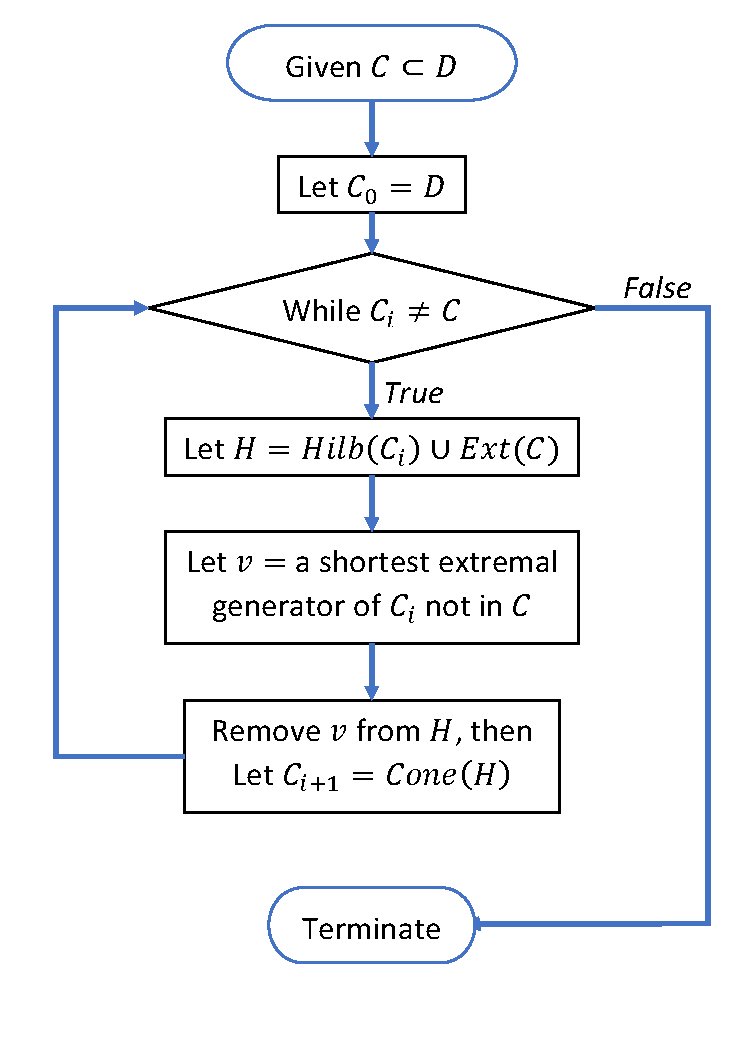
\includegraphics[width=.49\textwidth]{TopDownFC.pdf}
\caption{Flow chart for the \emph{Top Down} algorithm.}
\end{figure}
This algorithm uses Hilbert Descents to "shave" $D$ down to $C$.


\begin{enumerate}
\item Let $D_0 = D$, i.e., we set the initial cone to be the outer cone $D$.
\item Let $H = \mathrm{Hilb}(D_0)$, i.e., we collect the indecomposable elements of $L(D_0)$.
\item Let $D_1 = \mathrm{Cone}(H \takeaway \{v\})$, i.e., we take the conical hull of all the indecomposable elements of $L(D_0)$ after removing $v$ from the list.


\item While $D_i \neq C$, 
	\begin{enumerate}
	
		\item Let $H$ be a list containing the Hilbert basis of $D_{i}$. 
		\item Collect the set extremal generators of $D$ that are not in $C$ and collect these vectors into a list $E_{i} = \mathrm{ExtGen}(D_i) \cap C^c$.
		\item Loop through $E_{i}$ and record the lengths of each vector. Then choose one of the vectors with the smallest Euclidean norm from this list, call this $v_i$.
		\item Return $D_{i+1} = \mathrm{Cone}(\mathrm{Hilb}(D_i)\takeaway\{v_i\} \cup C)$, i.e., remove $v_i$ from the list $H$, and return the conical hull of $H \takeaway \{v_i\}$.
		
	\end{enumerate} 
\end{enumerate}


\subsection{Bottom Up}
We grow the inner cone to the outer cone by height-1 extensions. Previous results have shown that this method produces a cone more quickly than the \emph{Top Down} algorithm.

In order to describe the algorithm, we define a special type of polyhedron called a \emph{zonotope}:
\begin{definition}[Zonotope]
A zonotope is a set of points in $d$-dimensional space constructed from vectors $v_i$ by taking the sum of $a_iv_i$, where each  $a_i$ is a scalar between 0 and 1. Given $V = \{ v_1,\ldots, v_k\}$:
$$\mathrm{Zonotope(V)} = \{ x \in \R^d: x = a_1v_1 + \cdots + a_k v_k \text{ and } 0 \leq a_i \leq 1 \text{ for each } a_i \}.$$
\end{definition}
\begin{figure}[h]
\centering
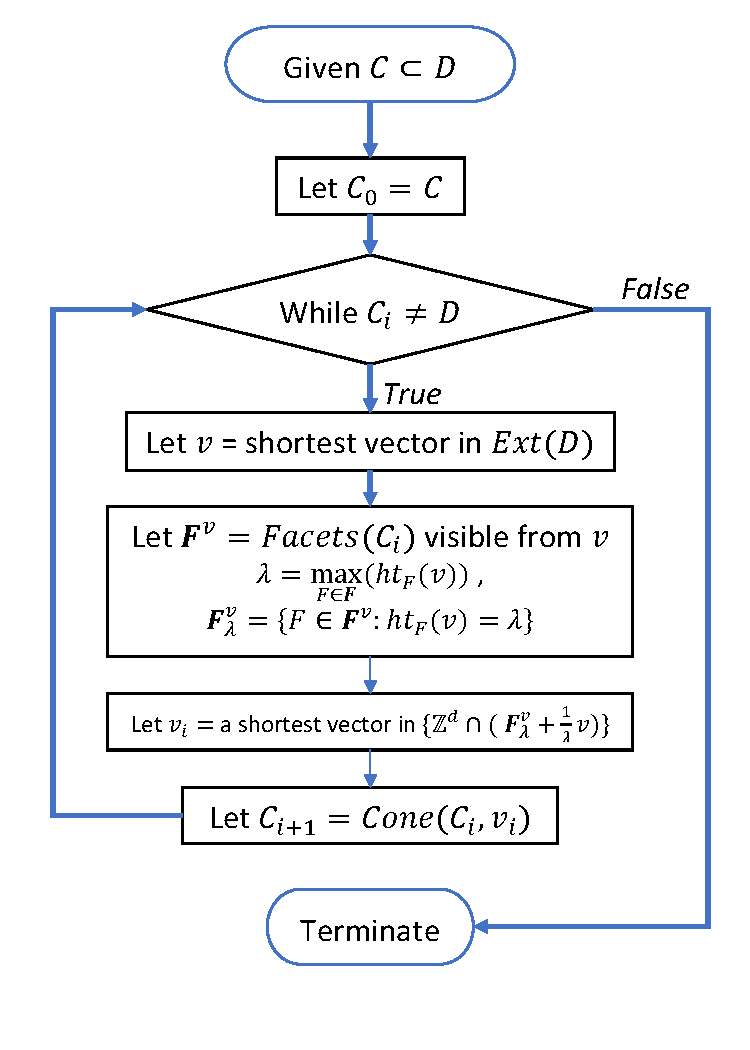
\includegraphics[width=.49\textwidth]{BottomUpFC.pdf}
\caption{Flow chart for the \emph{Bottom Up} algorithm.}
\end{figure}



\begin{enumerate}

\item Let $C_0 = C$.
\item While $C_i \neq D$:

\begin{enumerate}
\item Collect the set of facets of $C_i$  visible from $v$:
\begin{enumerate}
\item Let $\mathbb F^v$ be the set of facets of $C$ visible from $v$, i.e., $H_{\alpha}$ is a support hyperplane of $C$ associated with a facet $F$.
\item  $F$ is visible from $v$ if $C \subset H_{\alpha}^+ \implies v \subset (H_{\alpha}^+)^c$. Computationally, we can simply check that $C$ and $v$ have opposite signs when evaluated using $\alpha$; i.e., if $\alpha(c) < 0 $ for every $c \in C$, then $F$ is visible from $v$ if $\alpha(v) > 0$.
 
\end{enumerate}
\item Let $ht_{F}(v) = \alpha(v)$ given that $\alpha$ is the linear form associated with the support hyperplane of the facet $F$.
\item Let $\lambda = \displaystyle\max_{F \in \F}(ht_{F}(v))$. Collect the set $\F^v_\lambda = \{F \in \F^v: ht_{F}(v) = \lambda\}$. 
\item Shift this set $\F^v_{\lambda}$ along $\frac{1}{\lambda} v$, and find the shortest integer lattice point. Looping through each shifted facet $F$ in $\F^v_{\lambda}$:
	\begin{itemize}
	\item Computationally, we take the extremal generators of each facet $F$ and from a zonotope $Z_F$. Shift $Z_F$ by $\frac{1}{\lambda}v$.
	\item Once we have $Z_F + \frac{1}{\lambda}v$, collect the vectors $L(Z_F+\frac{1}{\lambda}v )$ and append this to a list $E_i$. 
\begin{remark}\label{zonotopelattice}
The zonotope $Z_F + \frac{1}{\lambda}v$ always contains at least one lattice element.
\end{remark}
	\end{itemize}
\item Loop through $E_i$ and find the shortest vector, called this $v_i$.
\item Return $C_{i+1} = \mathrm{Cone}(C \cup v_i)$. 
\end{enumerate}
\end{enumerate}





The two algorithms can be used alternatively, and we examine the difference of the two algorithms by comparing the number of elements of the Hilbert basis of each successive cone. 


\begin{lemma}
The \emph{Top Down} and \emph{Bottom Up} algorithms yield the same chain of cones in $\R^2$.
\end{lemma} 


\begin{figure}[h]
\begin{multicols}{2}
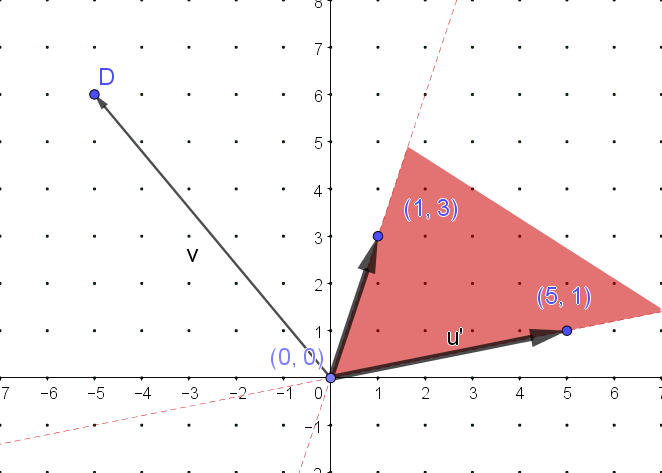
\includegraphics[width=.49\textwidth]{SimpleCone}
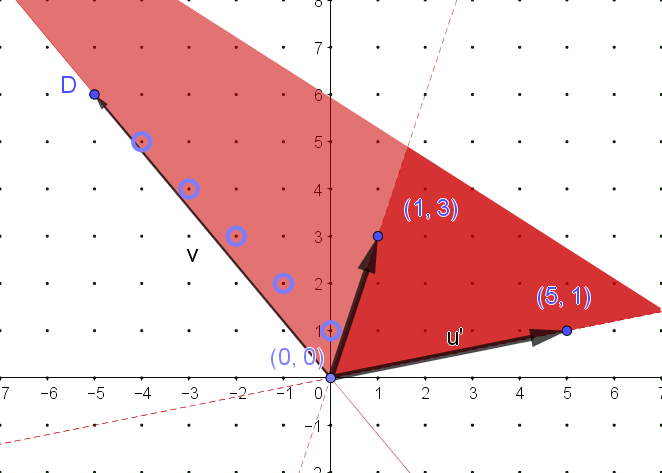
\includegraphics[width=.49\textwidth]
{SimpleCone2}
\end{multicols}

\caption{Demonstration of the \emph{Top Down} and \emph{Bottom Up} algorithms in $\R^2$.}
\end{figure}

Yet, for $d > 2$, in $\R^d$ the algorithms do not always generate the same cones, demonstrated in the data section below.




\section{Objects and Data Structure Overview}

\begin{figure}[h]
\centering
\includegraphics[width=.75\textwidth]{"Data Structure Picture"}
\caption{Visualization of Object-Oriented Design.}
\end{figure}
The object oriented version currently existing on \texttt{Github} allows for advantages over the procedural version in several ways. In particular, the Hilbert basis calculation for each cone used in the Top Down algorithm is computationally expensive, and the most elementary data structure in this design was created specifically to avoid doing multiple calculations on the same cone. 

Three central objects were created for this experiment, and here we present the essential attributes and methods of the code. The reader may find the source code in \textbf{Chapter~\ref{Source}}.

\begin{enumerate}
	
\item \texttt{cone\_chain\_element.py} Object file that contains a \texttt{SAGE} polyhedron object (which is our cone) and the associated data and methods:
	\begin{itemize}
	\item Essential Attributes:
		\begin{itemize}
		\item \texttt{cone, cone\_rays\_list}: The \texttt{SAGE} polyhedron object and the extremal generators of the cone.			
		\item \texttt{generation\_step, algorithm\_used}: to denote what step this cone was generated and what algorithm was used. 0 if initial cones. For algorithm used, the letter "i" denotes initial cone, "t" denotes top down, "b" denotes bottom up.
		\item \texttt{hilbert\_basis} Storing Hilbert basis of the cone in this object. This ensures that the calculation is only done once.
		\end{itemize}
	\item Essential Methods:
		\begin{itemize}
		\item \texttt{get\_hilbert\_basis(self)} Method to interface with the data in the object, with the logic to guarantee that \texttt{Normaliz} is used at most once for each \texttt{ConeChainElement} object.
		\item \texttt{output\_details(self)} Prints to terminal details about this particular cone. Used in other I/O methods elsewhere.
		\end{itemize}
	\end{itemize}
	
\item \texttt{cone\_chain.py} Object file that contains three lists of \texttt{ConeChainElements} designed to represent three valid cone poset chains. 
	\begin{itemize}
	\item Attributes:
		\begin{itemize}
		\item \texttt{inner\_cone, outer\_cone} the cones initializing the experiment.
		\item \texttt{top\_sequence}: first contains \texttt{outer\_cone}, then every cone generated by the \texttt{top\_down} algorithm.
		\item \texttt{bottom\_sequence}: first contains \texttt{inner\_cone}, then every cone generated by the \texttt{bottom\_up} algorithm.
		\item \texttt{cone\_chain}: generated only when the either \texttt{top\_down / bottom\_up} terminates, and arranges it so that the \texttt{inner\_cone} is the first element and the \texttt{outer\_cone} is the last element.
		\end{itemize}
	\item Methods:
		\begin{itemize}
		\item \texttt{top\_down} algorithm, implements Hilbert descends.
		\item \texttt{bottom\_up} algorithm, implements height-1 extensions.
		\end{itemize}
	\end{itemize}
\item \text{cone\_conjecture\_tester.py} Wrapper object that deals with all UI, creation/initialization of experiments, loading/saving operations. This also contains functions to generate graphs and save summaries.
\end{enumerate}


\end{document}

\chapter{Source Code} \label{Source}

%--------------------------------------------%
% Packages arranged by : Tsz Timmy Chan	     %
%                 Date : November 26th, 2016%
%--------------------------------------------%

\documentclass{TC}
\usepackage{TCcommon}

\title{TITLE HERE}	% Work Title Here.
\author{Tsz Timmy Chan}	% YOUR NAME HERE 

\usepackage[notes]{TCheader}
\usepackage{TCexamtitle}
%\renewcommand{\benediction}{" " - }
%\renewcommand{\quoteoftheday}{" " \\ - }
\begin{document}
Included here are code that is written in \texttt{Python} for this research, and they are also concurrently hosted on 


\begin{center}
\begin{minipage}{.75\textwidth}
\begin{mdframed}
\texttt{http://www.github.com/TimmyChan/ConeThesis}
\end{mdframed}
\end{minipage}
\end{center}

\texttt{cone\_tools.py} This file contains mathematical functions written for the project:
	\begin{itemize}
		\item \texttt{cone\_containment(C,D)}: Verifies C is contained in D
		\item \texttt{shortest\_vector(vectorlist), longest\_vector(vectorlist)}: Returns the shortest and longest vectors from a list, respectively.
		\item \texttt{make\_primitive(vectlist)}: Returns a primitive vector along the ray generated by some vector in $\Z^d$.
		\item \texttt{generate\_random\_vector(dim, rmax=10)}: Generates a random vector in $v \in \Z^d$ such that $\abs{v_i} \leq d$ and $v_d \geq 1$. The last condition is used to guarantee the following function always generates a cone contained in the halfspace $x_d > 0$, so it contains no lines. Using the previous function we always generate a random \emph{primitive} vector.
		
		\item \texttt{generate\_cone(dim, rmax=10,numgen=10), generate\_inner\_cone(outer)}: Generates a cone using random vectors constrained by the dimension (dim) and the random generation bounds. Numgen is the number of vectors used to generate the cone. The latter generates a cone that is guaranteed to be contained by the outer cone.
		
		\item \texttt{extremal\_generators\_outside\_inner\_cone(inner, outer)}: This is used to find a list of extremal generators at the beginning of the Top Down algorithm.
		
		\item \texttt{visible\_facets(cone,vect), facets\_with\_max\_lambda(visiblefacets,v)}: These are used in the Bottom Up algorithm.
		
		\item \texttt{vector\_sum(listofvectors), zonotope\_generators(vectlist)}: Generating a zonotope in $\Z^d$ using the power set of a set of vectors, then taking sum of each element of the power set, and adjoining the empty set as the origin.
				
	\end{itemize}

\newpage
\section{cone\_tools.py}
\input{"cone_tools.py.tex"}
\newpage
\section{cone\_chain\_element.py}
\input{"cone_chain_element.py.tex"}
\newpage
\section{cone\_chain.py}
\input{"cone_chain.py.tex"}
\newpage
\section{cone\_conjecture\_tester.py}
\input{"cone_conjecture_tester.py.tex"}
\end{document}

\chapter{Computational Results}
%--------------------------------------------%
% Packages arranged by : Tsz Timmy Chan	     %
%                 Date : November 26th, 2016%
%--------------------------------------------%

\documentclass{TC}
\usepackage{TCcommon}

\title{TITLE HERE}	% Work Title Here.
\author{Tsz Timmy Chan}	% YOUR NAME HERE 

\usepackage[notes]{TCheader}
\usepackage{TCexamtitle}
%\renewcommand{\benediction}{" " - }
%\renewcommand{\quoteoftheday}{" " \\ - }
\begin{document}



\section{Data Collection Technique}
We examine cones in dimension 4 and 5:
\begin{table}[h]
\centering
\begin{tabular}{c | c| c}
dimension & number of extremal generators & $k \in \Z: |x_i|< k$ \\ \hline
4 & (4,5) & 2 \\
5 & (5,6) & (1,2)
\end{tabular}
\caption{Conditions tested.}
\end{table}


The code was written in an object oriented fashion which allows for use in other python scripts. Thus, the experiments are generated in batch; each experiment is named "\{\} generators \{\} bound \{letter\}" where the first "\{\}" is the number of extremal generators and the latter is the bound on the absolute value on each coordinate. Files named with the same \{letter\} will have the same initial conditions. We run a fixed number of steps at the beginning, with a separate script that continues any existing experiment a fixed number of steps or loop for a fixed amount of time. The details of how the script looks can be found in the appendix.

We collect and record the number of steps taken for top down as well as bottom up for a particular pair of cones. Then we examine the Hilbert basis in the algorithmically generated poset chains. To study the complexity of the cones in the poset chain, we record the number of elements in the Hilbert basis, or $\#\Hilb(C)$ and also examine the Euclidean norm of the longest vector in the Hilbert basis of $C$. This information is presented in graphical form, using \texttt{figure} and \texttt{plot} functions in the standard Python package \texttt{pylab}.

Note that the way the graphs are arranged, the top down sequence begins with the "top" cone, or the "outer" cone. In contrast, the bottom up sequence begins with "bottom" or "inner" cone. 

Interestingly, some cones seem to terminate only on one of the algorithms!



\newpage


{
\singlespacing
\section{Data in dimension 4}
\subsection{4 generators 2 bound A}
\input{"4d 4 generators 2 bound A.tex"}
\newpage

\subsection{4 generators 2 bound B}
\input{"4d 4 generators 2 bound B.tex"}
\newpage

\subsection{4 generators 2 bound C}
\input{"4d 4 generators 2 bound C.tex"}
\newpage

\subsection{4 generators 2 bound D}
\input{"4d 4 generators 2 bound D.tex"}
\newpage

\subsection{4 generators 2 bound E}
\input{"4d 4 generators 2 bound E.tex"}
\newpage

\subsection{4 generators 2 bound F}
\input{"4d 4 generators 2 bound F.tex"}
\newpage

\subsection{4 generators 2 bound G}
\input{"4d 4 generators 2 bound G.tex"}
\newpage

\subsection{4 generators 2 bound H}
\input{"4d 4 generators 2 bound H.tex"}
\newpage

\subsection{4 generators 2 bound I}
\input{"4d 4 generators 2 bound I.tex"}
\newpage

\subsection{4 generators 2 bound J}
\input{"4d 4 generators 2 bound J.tex"}
\newpage



\subsection{5 generators 2 bound A}
\input{"4d 5 generators 2 bound A.tex"}
\newpage

\subsection{5 generators 2 bound B}
\input{"4d 5 generators 2 bound B.tex"}
\newpage

\subsection{5 generators 2 bound C}
\input{"4d 5 generators 2 bound C.tex"}
\newpage

\subsection{5 generators 2 bound D}
\input{"4d 5 generators 2 bound D.tex"}
\newpage

\subsection{5 generators 2 bound E}
\input{"4d 5 generators 2 bound E.tex"}
\newpage

\subsection{5 generators 2 bound F}
\input{"4d 5 generators 2 bound F.tex"}
\newpage

\subsection{5 generators 2 bound G}
\input{"4d 5 generators 2 bound G.tex"}
\newpage

\subsection{5 generators 2 bound H}
\input{"4d 5 generators 2 bound H.tex"}
\newpage

\subsection{5 generators 2 bound I}
\input{"4d 5 generators 2 bound I.tex"}
\newpage

\subsection{5 generators 2 bound J} \label{fail1}
\input{"4d 5 generators 2 bound J.tex"}
\newpage



\section{Data in dimension 5}
\subsection{5 generators 1 bound A}
\input{"5d 5 generators 1 bound A.tex"}\newpage

\subsection{5 generators 1 bound B}
\input{"5d 5 generators 1 bound B.tex"}
\newpage

\subsection{5 generators 1 bound C}
\input{"5d 5 generators 1 bound C.tex"}
\newpage

\subsection{5 generators 1 bound D}
\input{"5d 5 generators 1 bound D.tex"}
\newpage

\subsection{5 generators 1 bound E}
\input{"5d 5 generators 1 bound E.tex"}
\newpage

\subsection{5 generators 1 bound F}
\label{fail3}
\input{"5d 5 generators 1 bound F.tex"}
\newpage

\subsection{5 generators 1 bound G}
\input{"5d 5 generators 1 bound G.tex"}
\newpage

\subsection{5 generators 1 bound H}
\input{"5d 5 generators 1 bound H.tex"}
\newpage

\subsection{5 generators 1 bound I}
\label{fail4} %DOUBLE FAIL
\input{"5d 5 generators 1 bound I.tex"}
\newpage

\subsection{5 generators 1 bound J}
\input{"5d 5 generators 1 bound J.tex"}
\newpage




\subsection{6 generators 1 bound A}

\input{"5d 6 generators 1 bound A.tex"}
\newpage

\subsection{6 generators 1 bound B}

\input{"5d 6 generators 1 bound B.tex"}
\newpage

\subsection{6 generators 1 bound C}

\input{"5d 6 generators 1 bound C.tex"}
\newpage

\subsection{6 generators 1 bound D}
\input{"5d 6 generators 1 bound D.tex"}
\newpage

\subsection{6 generators 1 bound E}
\input{"5d 6 generators 1 bound E.tex"}
\newpage

\subsection{6 generators 1 bound F}
\input{"5d 6 generators 1 bound F.tex"}
\newpage

\subsection{6 generators 1 bound G}
\input{"5d 6 generators 1 bound G.tex"}
\newpage

\subsection{6 generators 1 bound H}
\input{"5d 6 generators 1 bound H.tex"}
\newpage

\subsection{6 generators 1 bound I}

\input{"5d 6 generators 1 bound I.tex"}
\newpage

\subsection{6 generators 1 bound J}
\input{"5d 6 generators 1 bound J.tex"}
\newpage




\subsection{5 generators 2 bound A}
\input{"5d 5 generators 2 bound A.tex"}
\newpage

\subsection{5 generators 2 bound B}
\input{"5d 5 generators 2 bound B.tex"}
\newpage

\subsection{5 generators 2 bound C}
\input{"5d 5 generators 2 bound C.tex"}
\newpage

\subsection{5 generators 2 bound D}
\input{"5d 5 generators 2 bound D.tex"}
\newpage

\subsection{5 generators 2 bound E}
\label{fail2}
\input{"5d 5 generators 2 bound E.tex"}
\newpage

\subsection{5 generators 2 bound F}
\label{fail3}
\input{"5d 5 generators 2 bound F.tex"}
\newpage

\subsection{5 generators 2 bound G}
\input{"5d 5 generators 2 bound G.tex"}
\newpage

\subsection{5 generators 2 bound H}
\input{"5d 5 generators 2 bound H.tex"}
\newpage

\subsection{5 generators 2 bound I}
\label{fail4} %double fail
\input{"5d 5 generators 2 bound I.tex"}
\newpage

\subsection{5 generators 2 bound J}
\input{"5d 5 generators 2 bound J.tex"}
\newpage




\subsection{6 generators 2 bound A}
\label{fail5} %double fail
\input{"5d 6 generators 2 bound A.tex"}
\newpage

\subsection{6 generators 2 bound B}
\label{fail6} %double fail
\input{"5d 6 generators 2 bound B.tex"}
\newpage


\subsection{6 generators 2 bound C}
\label{fail7} %double fail
\input{"5d 6 generators 2 bound C.tex"}
\newpage

\subsection{6 generators 2 bound D}
\input{"5d 6 generators 2 bound D.tex"}
\newpage

\subsection{6 generators 2 bound E}
\label{fail8} %double fail
\input{"5d 6 generators 2 bound E.tex"}
\newpage

\subsection{6 generators 2 bound F}
\label{fail9} %double fail
\input{"5d 6 generators 2 bound F.tex"}
\newpage

\subsection{6 generators 2 bound G}
\label{fail10} %double fail
\input{"5d 6 generators 2 bound G.tex"}
\newpage

\subsection{6 generators 2 bound H}
\input{"5d 6 generators 2 bound H.tex"}
\newpage

\subsection{6 generators 2 bound I}
\label{fail11} %double fail
\input{"5d 6 generators 2 bound I.tex"}
\newpage

\subsection{6 generators 2 bound J}
\input{"5d 6 generators 2 bound J.tex"}
\newpage
}
\section{Further Explorations using Alternating algorithm}
As some of the above experiments did not terminate as we expected, we device an alternating algorithm using a combination of the \texttt{bottom\_up} and \texttt{top\_down} algorithms. The results are recorded below. None of the initial conditions with non-terminating results terminated with this alternating method.

{
\singlespacing
\newpage
\subsection{5d 5 generators 2 bound I alternating}
\input{"5d 5 generators 2 bound I alternating.tex"}
\newpage

\subsection{5d 6 generators 2 bound A alternating}
\input{"5d 6 generators 2 bound A alternating.tex"}
\newpage

\subsection{5d 6 generators 2 bound C alternating}
\input{"5d 6 generators 2 bound C alternating.tex"}
\newpage

\subsection{5d 6 generators 2 bound E alternating}
\input{"5d 6 generators 2 bound E alternating.tex"}
\newpage

\subsection{5d 6 generators 2 bound F alternating}
\input{"5d 6 generators 2 bound F alternating.tex"}
\newpage

\subsection{5d 6 generators 2 bound G alternating}
\input{"5d 6 generators 2 bound G alternating.tex"}
\newpage

\subsubsection{5d 6 generators 2 bound I alternating}
\input{"5d 6 generators 2 bound I alternating.tex"}
\newpage
}

\end{document}


\chapter{Conclusion}

%--------------------------------------------%
% Packages arranged by : Tsz Timmy Chan	     %
%                 Date : November 26th, 2016%
%--------------------------------------------%

\documentclass{TC}
\usepackage{TCcommon}

\title{TITLE HERE}	% Work Title Here.
\author{Tsz Timmy Chan}	% YOUR NAME HERE 

\usepackage[notes]{TCheader}
\usepackage{TCexamtitle}
%\renewcommand{\benediction}{" " - }
%\renewcommand{\quoteoftheday}{" " \\ - }
\begin{document}
The data in dimension 4 and 5 both have examples of non-terminating sequences. The results in \textbf{subsections \ref{fail1}, \ref{fail2}, \ref{fail3}, \ref{fail4}, \ref{fail5}, \ref{fail6}, \ref{fail7}, \ref{fail8}, \ref{fail9}, \ref{fail10}, \ref{fail11}} show that the top down algorithm will demonstrate a roughly linear increase of the size of Hilbert basis as the number of steps in the algorithm increases. This makes it less and less likely as the number of
steps grows that we have a terminating process. This evidence suggests the negative
answer to questions (3) and (4) at the end of \textbf{section \ref{coneconjecturequestions}} 

Some of the experiments do not terminate on the top down algorithm, but terminate on the bottom up algorithm. This suggests that the bottom up algorithm moves in ”wider” steps than the top down algorithm. The expectation is further supported by the fact that when both procedures terminate, the bottom up algorithm does so in a fewer steps than the top down algorithm.


\section{Further Study}
The algorithms can see some further changes. For example, the extremal generator removed by the top down algorithm perhaps can be chosen based on some "greedy" algorithm instead, where we examine the volume of the cones of the possible choices before choosing. However, this may lead to worse computational efficiency, as at each step one would have to calculate the volume of a cone, usually represented as the volume of the parallelepiped created by the extremal rays. 


An exhaustive search of particular classes of cones, or cones in regions might become feasible if we can find a quick way to explicitly generate full dimensional cones in a particular region.

On the computer science side, modifying the project so that it is compatible with \texttt{Docker} would allow for computation on a stronger machine, which could provide more certainty towards the questions (3) and (4). 



\end{document}


%\appendix{Appendix A: Notation}
%
%--------------------------------------------%
% Packages arranged by : Tsz Timmy Chan	     %
%                 Date : November 26th, 2016%
%--------------------------------------------%

\documentclass{TC}
\usepackage{TCcommon}

\title{Notation}	% Work Title Here.
\author{Tsz Timmy Chan}	% YOUR NAME HERE 

\usepackage[notes]{TCheader}
\usepackage{TCexamtitle}
%\renewcommand{\benediction}{" " - }
%\renewcommand{\quoteoftheday}{" " \\ - }
\begin{document}
\begin{center}
\begin{tabular}{c|c}
\textbf{Notation} & \textbf{Definition}  \\ \hline \hline
$\Z, \R$ & The sets of Integers, Real numbers, respectively \\\hline
$\Z_+, \R_+$ & The set of non-negative integers and real numbers, respectively. \\\hline
$\mathrm{cone}(V)$ & The conical hull of $V$, where $V$ is a set of vectors.\\ 
\end{tabular}
\end{center}


\end{document}


\end{document}


%==============%
% Bibliography %
%==============%

% BibTex %
%\bibliographystyle{amsplain}
%\addcontentsline{toc}{chapter}{Bibliography}
%\singlespacing
%\bibliography{thesis}



%BibLatex :
\printbibliography


%--------------------------------------------%
% Packages arranged by : Tsz Timmy Chan	     %
%                 Date : November 26th, 2016%
%--------------------------------------------%

\documentclass{TC}
\usepackage{TCcommon}

\title{TITLE HERE}	% Work Title Here.
\author{Tsz Timmy Chan}	% YOUR NAME HERE 

\usepackage[notes]{TCheader}
\usepackage{TCexamtitle}
%\renewcommand{\benediction}{" " - }
%\renewcommand{\quoteoftheday}{" " \\ - }
\begin{document}

\begin{appendices}

The appendices include the source code for the following files:
\begin{itemize}
\item \texttt{experiment\_io\_tools.py} This is a small package of i/o scripts written for this experiment. 

\item \texttt{batch\_run\_experiments.py} This is a demonstration of how to create experiments using the \texttt{ConeConjectureTester} object

\item \texttt{batch\_continue.py} This is a demonstration of how to load and continue experiments already created.

\item \texttt{generate\_latex\_files.py} This is the script used to generate the data latex files.
\end{itemize}

\chapter{experiment\_io\_tools.py}
\input{"experiment_io_tools.py.tex"}

\chapter{batch\_run\_experiments.py}
\input{"batch_run_experiments.py.tex"}

\chapter{batch\_continue.py}
\input{"batch_continue.py.tex"}

\chapter{generate\_latex\_files.py}
\input{"generate_latex_files.py.tex"}
%
%--------------------------------------------%
% Packages arranged by : Tsz Timmy Chan	     %
%                 Date : November 26th, 2016%
%--------------------------------------------%

\documentclass{TC}
\usepackage{TCcommon}

\title{TITLE HERE}	% Work Title Here.
\author{Tsz Timmy Chan}	% YOUR NAME HERE 

\usepackage[notes]{TCheader}
\usepackage{TCexamtitle}
%\renewcommand{\benediction}{" " - }
%\renewcommand{\quoteoftheday}{" " \\ - }
\begin{document}


\begin{SAGE}
from sage.all import *
from sage.misc import *
#import PyNormaliz as PyNormaliz
import numpy as np
from Init import *

# Please note that to make a default cone in SAGE, one must now use 
# sage.geometry.cone.Cone(list), where list is a list of vectors.



INFINITYCORK = 10000




# One step in the loop, step 4 in the psuedocode 
# Assumes Intermediate is a SAGE default cone object.
def TOPDOWNstep(C,Intermediate,FILE=None,verbose=False):
	if verbose:
		def verboseprint(*args):
			for arg in args:
				print arg,
				if FILE <> None:
					FILE.write("\n"+str(arg))
			print
	else:
		verboseprint = lambda *a: None 

	# Collect the set of extremal generators of the intermediate cone that is not in C
	ExtremalNotinC = ExtremalGeneratorNotContainedbyInnerCone(C, Intermediate,FILE,verbose)

	
	VectorToRemove = shortestvector(ExtremalNotinC)
	verboseprint("Vector norms: {}".format([r.norm() for r in ExtremalNotinC]))
	verboseprint("Vector to remove = {} and its norm = {}".format(VectorToRemove,VectorToRemove.norm()))

	IntermediateHB = list(Intermediate.integral_points_generators()[1])
	#verboseprint(IntermediateHB)
	#verboseprint("Hilbert Basis of Intermediate Cone: \n {}".format(IntermediateHB))

	IntermediateHB.remove(VectorToRemove)
	NewGenerators = IntermediateHB + list([list([long(i) for i in ray]) for ray in C.rays()])
	#verboseprint("Forming new cone with: \n{}".format(NewGenerators))
	verboseprint("Forming cone with {} vectors in Hilbert Basis of D + Extremal Generators of C.".format(len(NewGenerators)))
	return Polyhedron(rays=NewGenerators,backend='normaliz')
	


def TOPDOWNtrial(C,D,FILE,verbose=False):
	if verbose:
		def verboseprint(*args):
			for arg in args:
			   print arg,
			   FILE.write("\n"+str(arg))
			print
	else:
		verboseprint = lambda *a: None 
	
	numC = len(C.rays()) 	# number of extremal generaters in C
	dim = C.dim()			# ambient dimension (since C is assumed full dimension)
	# STEP 1: Set the "intermediate cone" to be D at the first step.
	IntermediateCone = D # IntermediateCone is a Polyhedron with normaliz backend


	if verbose and dim <= 3:
		plotCD(C,D,FILE,"INITIAL CONDITION.png")
		#PLOT = C.plot(point=False, line=False, polygon=(0,0,1)) + D.plot(point=False,line='red',polygon=False)
		#PLOT.save(FILE.name[:-4] + "INITIAL CONDITION.png")

	# STEP 4: look in the definition of TOPDOWNstep.
	counter = 0
	
	IntermediateCone = D
	if verbose and dim <= 3:
		plotCD(IntermediateCone,D, FILE,"STEP {}.png".format(counter))
		#PLOT = D.plot() + C.plot()
		#PLOT.save(FILE.name[:-4] + "STEP {}.png".format(counter))
	

	while (not C ==IntermediateCone):
		if verbose:
			stepcheck(TOPDOWNstep(C,IntermediateCone,None),IntermediateCone)
		IntermediateCone = TOPDOWNstep(C,IntermediateCone,FILE,verbose)
		counter = counter + 1
		if verbose and dim <= 3:
			plotCD(IntermediateCone,D,FILE,"STEP {}.png".format(counter))
			#PLOT = IntermediateCone.plot(point=False, line=False, polygon=(0,0,1)) + D.plot(point=False, line='red', polygon=False)
			#PLOT.save(FILE.name[:-4] + "STEP {}.png".format(counter))
		verboseprint("#########################################")
		verboseprint("Finished Step {} - Original number of extremal rays: {}, Now: {}".format(counter,numC, len(IntermediateCone.rays())))
		
		if not D.intersection(IntermediateCone) == IntermediateCone:
			print("ERROR: Intermediate Cone not in D")
			FILE.write("\nERROR: Intermediate Cone not in D")
			
			break
		if not IntermediateCone.intersection(C) == C:
			FILE.write("\nERROR: C not in Intermediate Cone")
			break
		#if not D.contains(IntermediateConeSAGE) or not IntermediateConeSAGE.contains(C):
		#	print("ERROR: D.contains(IntermediateConeSAGE) = {} \nIntermediateConeSAGE.contains(C) = {}".format(D.contains(IntermediateConeSAGE),IntermediateConeSAGE.contains(C)))
		#	break
		if counter >= INFINITYCORK:
			print("ERROR: At step {}, possible candidtate for nonterminating case...".format(counter))
			FILE.write("\nERROR: At step {}, possible candidtate for nonterminating case...".format(counter))
			PrintCD(C,D,FILE)
			break
	if C == IntermediateCone:
		verboseprint("\n Intermediate Cone = \n{}\n Goal Cone = \n{}\n Initial Cone = \n{}\n\tFinished in {} steps. ".format(IntermediateCone.rays_list(),C.rays_list(),D.rays_list(),counter))
		#FILE.write("\n Intermediate Cone = \n{}\n Goal Cone = \n{}\n Initial Cone = \n{}\n\tFinished in {} steps. ".format(IntermediateCone.rays_list(),C.rays_list(),D.rays_list(),counter))
	return counter, C, D 
\end{SAGE}


\end{document}


%
%--------------------------------------------%
% Packages arranged by : Tsz Timmy Chan	     %
%                 Date : November 26th, 2016%
%--------------------------------------------%

\documentclass{TC}
\usepackage{TCcommon}

\title{TITLE HERE}	% Work Title Here.
\author{Tsz Timmy Chan}	% YOUR NAME HERE 

\usepackage[notes]{TCheader}
\usepackage{TCexamtitle}
%\renewcommand{\benediction}{" " - }
%\renewcommand{\quoteoftheday}{" " \\ - }
\begin{document}
\begin{SAGE}
from sage.all import *
from sage.misc import *
#import PyNormaliz as PyNormaliz
import numpy as np
from Init import *

# Function takes on C, v: v is external to C
# 	Returns a list of facets [f1,f2,...,fn], where each f_i is visible WRT v
def facetsVisiblefromV(C,v):

	if C.contains(v):
		return None
	else:
		#print("v = {}\n C = \n{}".format(v,C.rays_list()))
		numfacets = len(C.faces(C.dim()-1)) # counts the number of facets of codimension 1

		facets = C.faces(C.dim()-1)
		#print("Number of facets of C = {} = {}".format(numfacets,len(facets)))
		#print facets
		visiblefacets = []
		for facet in facets:
			#print("Facet {}:".format(facets.index(facet)))
			facetIneq = facet.ambient_Hrepresentation(0)
			#print("\tambient halfspace {}".format(facetIneq))
			facetIsVisibile = (facetIneq.eval(vector(v)) < 0)
			#print facetIneq.eval(vector(v))
			#print("\trays = {}".format(facet.as_polyhedron().rays_list()))
			if facetIsVisibile:
				#print("\t Facet {} visible!".format(facets.index(facet)))
				visiblefacets.append(facet)
		#print visiblefacets
		return visiblefacets


def facetsMaxLambda(visiblefacets,v):
	return max(visiblefacets, key = lambda x: abs(x.ambient_Hrepresentation(0).eval(vector(v))))


# takes a list of vectors of the same dimension
# returns a vector that is the termwise sum of each vector in the list.

def vectorsum(listofvectors):
	length = len(listofvectors)
	dim = len(listofvectors[0])
	summand = [0 for i in range(dim)]
	for i in range(length):
		for d in range(dim):
			summand[d] = summand[d] + listofvectors[i][d]
	return summand
# accepts a list of vectors, assumes they're all same dimension.
# returns a list of vectors that are the vertices of a zonotope generated by the list inputted.
def zonotope(vectlist):
	# First create the powerset of the list	and remove the empty set.
	dimension = len(vectlist[0])
	combo = list(powerset(vectlist))
	combo.remove([])
	combo.append([[0 for i in range(dimension)]])
	#print combo
	zonogens = [vectorsum(c) for c in combo]
	#print zonogens
	#return Polyhedron(vertices=zonogens,backend='normaliz')
	return zonogens


def BOTTOMUPstep(C,v,FILE=None,verbose=False):
	if verbose:
		def verboseprint(*args):
			for arg in args:
				print arg,
				if FILE <> None:
					FILE.write("\n"+str(arg))
			print
	else:
		verboseprint = lambda *a: None 
	# dimension of the space must be the length of each vector
	dimension = len(v)
	visibleFacetsofIntermediate = facetsVisiblefromV(C,v)

	visiblemaxlambdaFacet = facetsMaxLambda(visibleFacetsofIntermediate, v)

	generators =  visiblemaxlambdaFacet.as_polyhedron().rays_list()
	#print("generators of visible facet with max lambda = {}".format(generators))
	
	#print("generators of parallelopiped: {}".format(paragens))
	zonotopeGenerators = zonotope(generators)

	ShiftFactor = 1/ abs(visiblemaxlambdaFacet.ambient_Hrepresentation(0).eval(vector(v)))

	#print("Lambda = {}".format(ShiftFactor))

	ShiftedVertex = [ShiftFactor*i for i in v]

	#print("Lambda v = {}".format(ShiftedVertex))
	#shiftedGenerators = [[gen[i] + ShiftedVertex[i] for i in range(dimension)] for gen in paragens]
	shiftedGenerators = [[gen[i] + ShiftedVertex[i] for i in range(dimension)] for gen in zonotopeGenerators]

	shiftedGenerators.append(ShiftedVertex)


	#print shiftedGenerators


	zono = Polyhedron(vertices=shiftedGenerators,backend='normaliz')
	#print zono
	integralpoints = list(zono.integral_points())
	#print integralpoints
	shortestIntegralPoint = shortestvector(integralpoints)
	verboseprint("Returning the convex hull of Intermediate with {}...".format(shortestIntegralPoint))
	return C.convex_hull(Polyhedron(rays=[shortestIntegralPoint],backend='normaliz'))

def BOTTOMUPtrial(C,D,FILE=None,verbose=False):
	if verbose:
		def verboseprint(*args):
			for arg in args:
				print arg,
				if FILE <> None:
					FILE.write("\n"+str(arg))
			print
	else:
		verboseprint = lambda *a: None 
	
	# Cone for interations
	Intermediate = C 

	# loop through each extremeal vector
	vlist = ExtremalGeneratorNotContainedbyInnerCone(Intermediate,D)
	counter = 0
	while vlist <> []:
		# if the list is empty, we're done. Print the list to show where we are...
		verboseprint("Extremal generators of D not in Intermediate: {}".format(vlist))
		# work on the longest vector first
		longestv = longestvector(vlist)
		counter = counter + 1
		if verbose:
			printseparator()
		verboseprint("Step {}".format(counter))
		# iterate through the algorithm once. 
		Intermediate = BOTTOMUPstep(Intermediate,longestv,FILE,verbose)
		# collect the list of extremal generators not in C again
		vlist = ExtremalGeneratorNotContainedbyInnerCone(Intermediate,D)

	return counter, C, D
\end{SAGE}


\end{document}


\end{appendices}


\end{document}

\end{document}
